\documentclass[a4paper,10pt]{article}
\usepackage{fancyhdr}
\fancyhead[L,C]{}
\fancyhead[R]{2020-0462-4}
\fancyfoot[L,R]{}
\fancyfoot[C]{\thepage}
\renewcommand{\headrulewidth}{0.4pt}

\usepackage{geometry}
\newgeometry{textwidth=16cm}
\usepackage{amsfonts}
\usepackage{amssymb}
\usepackage[T1]{fontenc}
\usepackage[utf8]{inputenc}
\PassOptionsToPackage{defaults=hu-min}{magyar.ldf}
\usepackage[magyar]{babel}
\setcounter{secnumdepth}{5}
\usepackage{graphicx}
\usepackage{multirow}
\usepackage{nowidow}[all]
\usepackage{pdfpages}

%\pagestyle{myheadings}
%\markboth{}{2020-0462-4}


\newcommand{\mksz}{Motoros Könnyűrepülő Szövetség\ }

\title{%
    \textbf{ÜZEMBENTARTÓI ZÁRÓJELENTÉS} \\
    \vspace*{36pt}
    \textbf{KBSZ 2020-0462-4 számon nyilvántartott\\
    LÉGIKÖZLEKEDÉSI BALESET}\\
    \vspace*{24pt}
    Esztergom repülőtér\\
    \vspace*{24pt}
    2020.09.16. 09:45\\
    \vspace*{24pt}
    Apollo C15TN\\
    06-25\\
    \vspace*{6cm}
    \thanks{\normalsize{A szakmai vizsgálat célja a 
légiközlekedési baleset és repülőesemény 
okának feltárása és a hasonló esetek megelőzése érdekében szükséges szakmai 
intézkedése kezdeményezése, valamint javaslatok megtétele. A szakmai 
vizsgálatnak semmilyen formában nem célja a vétkesség vagy a felelősség 
vizsgálata és megállapítása.}}
}


\author{}
\date{}

\begin{document}


\maketitle
\pagebreak
\pagestyle{fancy}
\tableofcontents
\listoffigures
\pagebreak

%\begin{abstract}
%A vizsgálati jelentés a 2020.09.16-án az LHEM -- Esztergom repülőtéren (id. 
%Rubik Ernő repülőtér) történt légiközlekedési baleset okainak feltárására, a 
%jövőben hasonló okból bekövetkező események elkerülése érdekében készült.
%\\
%
%A balesetben egy sárkányrepülőgép gyakorló légtérrepülési feladat 
%végrehajtása után, leszállás végrehajtása közben szenvedett balesetet. 
%Az esemény során személyi sérülés nem történt. A baleset következtében a 
%sárkányrepülőgép súlyosan megrongálódott, egyéb dologi kár nem keletkezett.
%\\
%\end{abstract}

\pagebreak


\section*{A vizsgálat üzemeltetői hatáskörbe történő utalása}
Az \textbf{Innovációs és Technológiai Minisztérium Közlekedésbiztonsági 
Szervezete} az esemény bejelentését követően a 2005. évi CLXXXIV. törvény 20.§ 
(1) bekezdése alapján, a \textit{KBSZ/83715-3/2020-ITM} levelében a 
Motoros Könnyűrepülő Szövetség hatáskörébe utalta.

Az üzembentartói vizsgálatról készített jelentést a repülőesemények szakmai 
vizsgálatának, valamint az üzembentartói vizsgálat részletes szabályairól szóló 
70/2015. (XII. 1.) NFM rendelet  10. §-a alapján, a felhívás kézbesítésétől 
számított 60 napon kell megküldeni a kbszrepules@itm.gov.hu elektronikus 
levélcímre.\\

\begin{tabular}{ll}
  -- Az esemény időpontja:& 2020.09.16. 09:45LT\\
  -- Az esemény helyszíne:& Esztergom (LHEM)\\
  -- KBSZ nyilvántartási száma:& 2020-0462-4\\
  -- Légijármű lajstromjele / azonosítója:& 06-25\\
\end{tabular}

\section*{Meghatározások és rövidítések}
\paragraph*{KBSZ} Közlekedésbiztonsági Szervezet
\paragraph*{Kbvt.} A légi-, a vasúti és a víziközlekedési balesetek és egyéb 
közlekedési események szakmai vizsgálatáról szóló 2005. évi CLXXXIV. 
törvény
\paragraph*{ITM} Innovációs és Technológiai Minisztérium
\paragraph*{NFM} Nemzeti Fejlesztési Minisztérium
\paragraph*{Vb.} Vizsgálóbizottság
\paragraph*{LT} Local Time (helyi idő)
\pagebreak

\section*{Az esemény összefoglalása}
\begin{tabular}{|l|l|l|}
\hline
\multicolumn{2}{|l|}{Esemény kategóriája} & légiközlekedési baleset\\ \hline
\multirow{7}{3cm}{Légijármű}
    & gyártója & Halley Kft.\\ \cline{2-3}
    & típusa & Apollo Jet Star C15TN\\ \cline{2-3}
    & azonosító jele & 06-25\\ \cline{2-3}
    & gyári száma & 290304\\ \cline{2-3}
    & tulajdonosa & Globépterv Kft.\\ \cline{2-3}
    & üzembentartója & magánszemély\\ \cline{2-3}
    & bérlője & nincs\\ \cline{2-3}
\hline
\multirow{2}{3cm}{Esemény}
    & napja és időpontja & 2020.09.16. 09:45LT\\ \cline{2-3}
    & helye & Esztergom N$47^o 45' 42''$ E$18^o 44' 06''$\\ \cline{2-3}
\hline
\multirow{3}{3cm}{Esemény kapcsán}
    & elhunytak száma & 0\\ \cline{2-3}
    & súlyos sérültek száma & 0\\ \cline{2-3}
    & könnyű sérültek száma & 0\\ \cline{2-3}
\hline
\multicolumn{2}{|l|}{Légijármű rongálódásának mértéke} & szárny 100\%, trike 
30\%\\ \hline
\end{tabular}

\section*{Az esemény bejelentése}
A KBSZ ügyeletére az eseményt 2020.09.16-án 10:04 körül a repülőtér vezetője 
dr. Siklósi Zoltán jelentette be. a \mksz  elnöke Szikora György az esemény 
bejelentési tájékoztatás figyelembevételével az eseményt ugyan ezen a napon 11 
órakor megerősítette.

\section*{Vizsgálóbizottság}
A KBSZ \textit{KBSZ/83715-3/2020-ITM} iktatószámú levele alapján a 
repülőesemény szakmai kivizsgálását a \mksz hatáskörébe utalta.\\A \mksz Vb. 
elnöke Kovács József.

\section*{Az eseményvizsgálat áttekintése}
A légijármű vezetője gyakorlatban tartó légtérrepülési feladatot hajtott végre.
Indulási hely: Esztergom repülőtér. Tervezett leszállóhely: Esztergom repülőtér.

A tervezett feladat végrehajtásához a személyi (egészségi állapot), tárgyi 
(repülőeszköz alkalmassága, repülés előtti ellenőrzés és dokumentálás), 
valamint a meteorológiai (szélerősség, látástávolság) feltételek megfeleltek. 
A légtérrepülés eseménymentes befejezése után a leszálláshoz a 20-es pálya 
harmadik fordulópontjára helyezkedett be. Viszonylag nagy sebességgel a 
pályaküszöb előtt, egyenetlen talajon ért földet, majd elpattant és visszaesett.

\section*{A vizsgálat adatai}
A KBSZ ügyeletére az eseményt 2020.09.16-án 10:04-kor az Esztergom repülőtér 
vezetője dr. Siklósi Zoltán jelentette be.
\\

A KBSZ a légiközlekedési balesetet 2020-0462-4 számon iktatta és a szakmai 
vizsgálatot a \mksz hatáskörébe utalta.Jelen zárójelentés-tervezet a helyszíni 
szemle és a pilóta nyilatkozata alapján készült.

\section{Ténybeli információk}
\subsection{A repülés lefolyása}
A pilóta, aki maga is motoros sárkányrepülő oktató, megfelelő szakmai 
tapasztalattal és a repülőtér mikroklímai ismeretével rendelkezett. Az 
eseménymentes légtérrepülési feladat végrehajtása után a 20-es pálya 3. 
fordulópontjára helyezkedett, majd a 4. fordulópont után folytatta az 
ereszkedést. A siklópálya megtörése után a repülő eszköz váratlanul 
megsüllyedt, és nagy sebességgel a repülőtér munkaterületén kívül ért földet. A 
nagy sebességű és egyenetlen területre történő földetérés során a repülőeszköz 
súlyosan megsérült. A repülő esemény Esztergom közigazgatási területén belül, 
Esztergom repülőtéren 
nappal, jó látási viszonyok között történ.

\subsection{Személyi sérülés}
Az esemény kapcsán személyi sérülés nem történt.

\subsection{Légi jármű sérülése}
A baleset során a motoros sárkányrepülőgép trikejának orrfutója kitört, a trike 
műgyanta burkolata eltörött. A légcsavar egyik tollát a sordronyzat 
elvágta. A durva földetérés miatt a szárny erőteljes lefelé irányuló mozgását a 
felső keresztkör sodronyzata az árboc felé továbbította, ami az erőhatás 
következtében elhajlott.
Az árboc elhajlása miatt a felső körök meglazultak, és az 
immár laza felső hosszkör a forgó légcsavar síkjába került. A légcsavar tolla 
elérte a laza felső hosszkört, megrántotta. A rántás következtében a gerinc 
megroppant, megsérült a kereszttartó, valamint a vitorla anyaga az erőhatás 
következtében felhasadt.
A repülőeszköz sérüléseit a 4. számú fénykép melléklet tartalmazza.

\subsection{Egyéb kár}
A repülőesemény kapcsán a repülőeszköz sérülésén kívül egyéb kár nem 
keletkezett.

\subsection{Személyzet adatai}
\subsubsection{A repülőeszköz parancsnoka}
\begin{tabular}{|l|l|l|}
\hline
 \multicolumn{2}{|l|}{Kora, neme} & 62 év, féri\\ \hline
 \multirow{4}{3cm}{Szakszolgálati engedélyének érvényessége}
    & Szakmai & 2022.02.26.\\ \cline{2-3}
    & Egészségügyi & Class 2; 2021.02.26.\\ \cline{2-3}
    & Képesítései & Motoros sárkányrepülő pilóta\\ \cline{2-3}
    & Jogosításai & Motoros sárkányrepülő oktató\\ \cline{2-3}
 \hline 
 \multirow{4}{3cm}{Repült ideje}
    & Összesen & 301 óra 03 perc\\ \cline{2-3}
    & Megelőző 30 napon & 02 óra 39 perc\\ \cline{2-3}
    & Megelőző 7 napban & 0 óra 0 perc\\ \cline{2-3}
    & Megelőző 24 órában & 0 óra 0 perc\\ \cline{2-3}
 \hline
 \multicolumn{2}{|l|}{Éves, légijármű kategóriánként összesen} & 19 óra 47 
perc\\ \hline
 \multicolumn{2}{|l|}{Az érintett típuson összesen} & 119 óra 45 perc\\ \hline
\end{tabular}

\subsubsection{A repülőeszköz adatai}
\subsubsection{Légialkalmassági bizonyítvány érvényessége}
A repülő eszköz légialkalmassági bizonyítványának érvényessége 2021.05.20. (2. 
számú melléklet)

\subsubsection{Általános adatok}
\begin{tabular}{|l|l|}
 \hline
 Repülőeszköz típusa & motoros sárkányrepülő\\ \hline
 szárny típusa & Apollo C15TN\\ \hline
 trike típusa & Apollo Jet Star GT\\ \hline
 szárny gyártási száma & 290304\\ \hline
 szárny gyártási éve & 2004\\ \hline
 trike gyártási száma & 290304\\ \hline
 trike gyártási éve & 2004\\ \hline
 motor típusa & Simonini Viktor 2\\ \hline
 motor gyártási száma & V265\\ \hline
\end{tabular}

\subsection{Meteorológia adatok}
A pilóta nyilatkozata alapján \textit{,,\dots Az időjárási körülményekről - a 
tervezett légtérrepülési feladathoz - meggyőződtem, tájékozódtam\dots ''}\\
(A pilóta nyilatkozatát a 3. számú melléklet tartalmazza.)

A meteorológiai előrejelzés alapján az esemény napján dél felől fátyolfelhők 
érkeztek, a kissé szűrt napsütés és kevés gomolyfelhő képződés mellet 
csapadék nem volt várható. Az előrejelzés szerint az ország középső és 
a délkeleti részén megélénkülő, néhol megerősödő délkeleti szélre, 27-32 
fok legmagasabb nappali hőmérsékletre lehetett számítani.

\subsection{Navigációs berendezések}
Navigációs berendezések az esemény lefolyására nem voltak hatással, ezért 
részletezésük nem szükséges.

\subsection{Összeköttetés}
Kommunikációs berendezések az esemény lefolyására nem voltak hatással, ezért 
részletezésük nem szükséges.

\subsection{Repülőtéri adatok}
Esztergom repülőtér adatai:\\
Esztergom közigazgatási területén belül, WGS 84 koordináta rendszerben megadva 
$N47^o 45' 42''$ $E18^o 44' 06''$ $80\times1000m$ pályairány $020/200$.
A repülőtér térképe \apageref{LHEM}. oldalon \aref{LHEM} ábrán látható.
\begin{figure}[ht!]
\centering
 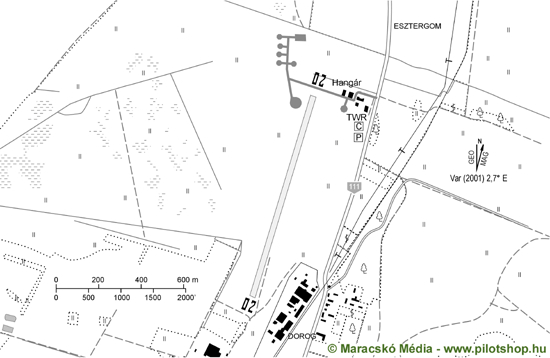
\includegraphics[width=10cm]{kepek/LHEM}
 \caption{Esztergom repülőtér}\label{LHEM}
 
\end{figure}


\pagebreak
\subsection{Légijármű adatrögzítő}
A repülőeszközön adatrögzítő nem volt.

\subsection{Repülőeszköz sérülésére vonatkozó adatok}
A repülő eszköz szárnya a baleset következtében javíthatatlanul megsérült, míg 
a trike sérülesinek becsült météke 30\% körülire tehető.\\
A repülőeszköz sérüléseit a 4. számú melléklet tartalmazza.

\subsection{Orvosi és igazságügyi-orvosszakértői vizsgálatok adatai}
A repülőesemény kapcsán személyi sérülés nem történt, ezért a Vb. orvosi és 
igazságügyi-orvosszakértői vizsgálatot nem végeztetett.

\subsection{Tűz}
A repülőesemény kapcsán tűz nem keletkezett.

\subsection{Túlélés lehetősége}
Személyi sérülés nem történt.

\subsection{Próbák és kísérletek}
A Vb. próbákat, kísérleteket nem végzett.

\subsection{Érintett szervezetek jellemzése}
Az érintett szervezetek jellemzői az esemény bekövetkezésére nem voltak 
hatással, ezért azok részletezése nem szükséges.

\subsection{Kiegészítő adatok}
A Vb. a fenti tényadatokon kívül a következtetések levonása és biztonsági 
ajánlások megtétele szempontjából egyéb körülményt nem tart lényegesnek, ezért 
további adatok nem kíván ismertetni.

\subsection{Hasznos és hatékony kivizsgálási módszerek}
A kivizsgálás során az általánostól eltérő módszerek alkalmazására nem volt 
szükség.

\section{Elemzés}
A légtérrepülési feladatra történő felkészülés repülésbiztonsági szempontból az 
előírásoknak megfelelt. A légtérrepülési feladat végrehajtása közben 
repülésbiztonságot érintő esemény nem történt. A leszállóhely, Esztergom 
repülőtér megközelítése a szabályoknak megfelelt. A pilóta a leszálló 
pályasíkot kis magasságban törte meg. A repülőeszköz váratlanul megsüllyedt, és 
nagy sebességgel, egyenetlen talajon a repülőtér munkaterületén kívül ért 
földet.

A repülőeszköz sérülését a nagysebességű, egyenetlen talajra történő leszállás 
okozta. A repülőeszköz váratlan megsüllyedését okozhatta szélnyírás, leáramlás, 
és egy esetleges turbulencia is.

\section{Következtetések}
\subsection{A repülőesemény bekövetkezésével közvetlen összefüggésbe hozható 
ténybeli megállapítások}
A repülőeszköz pilótája nagyon kis magasságon törte meg a leszálló pályasíkot, 
ennek következtében nem tudta korrigálni a váratlan megsüllyedést és nagy 
sebességgel egyenetlen talajon a repülőtér munkaterületén kívül ért földet.

\section{Biztonsági ajánlás}
A vonatkozó szabályok betartásával az ilyen repülő események elkerülhetők, 
ezért biztonsági ajánlás kiadására az esemény ismertetésén túl nincs szükség.

\vspace{2cm}

Budapest, 2020. október 11.

\vspace{2cm}

\begin{tabular*}{16cm}{ccc}
 Kovács József&\hspace{3cm} &Szikora György\\
 \mksz&\hspace{3cm} &\mksz\\
 Vb. elnök&\hspace{3cm} &elnök\\
\end{tabular*}

\pagebreak
\section{Mellékletek}
\begin{enumerate}
 \item számú melléklet -- Pilóta és a repülőeszköz dokumentumai
 \item számú mellékelt -- Légialkalmassági felülvizsgálati tanúsítvány
 \item számú melléklet -- Pilóta nyilatkozata
 \item számú melléklet -- A repülő eszköz sérülései - fényképek
\end{enumerate}

\pagebreak

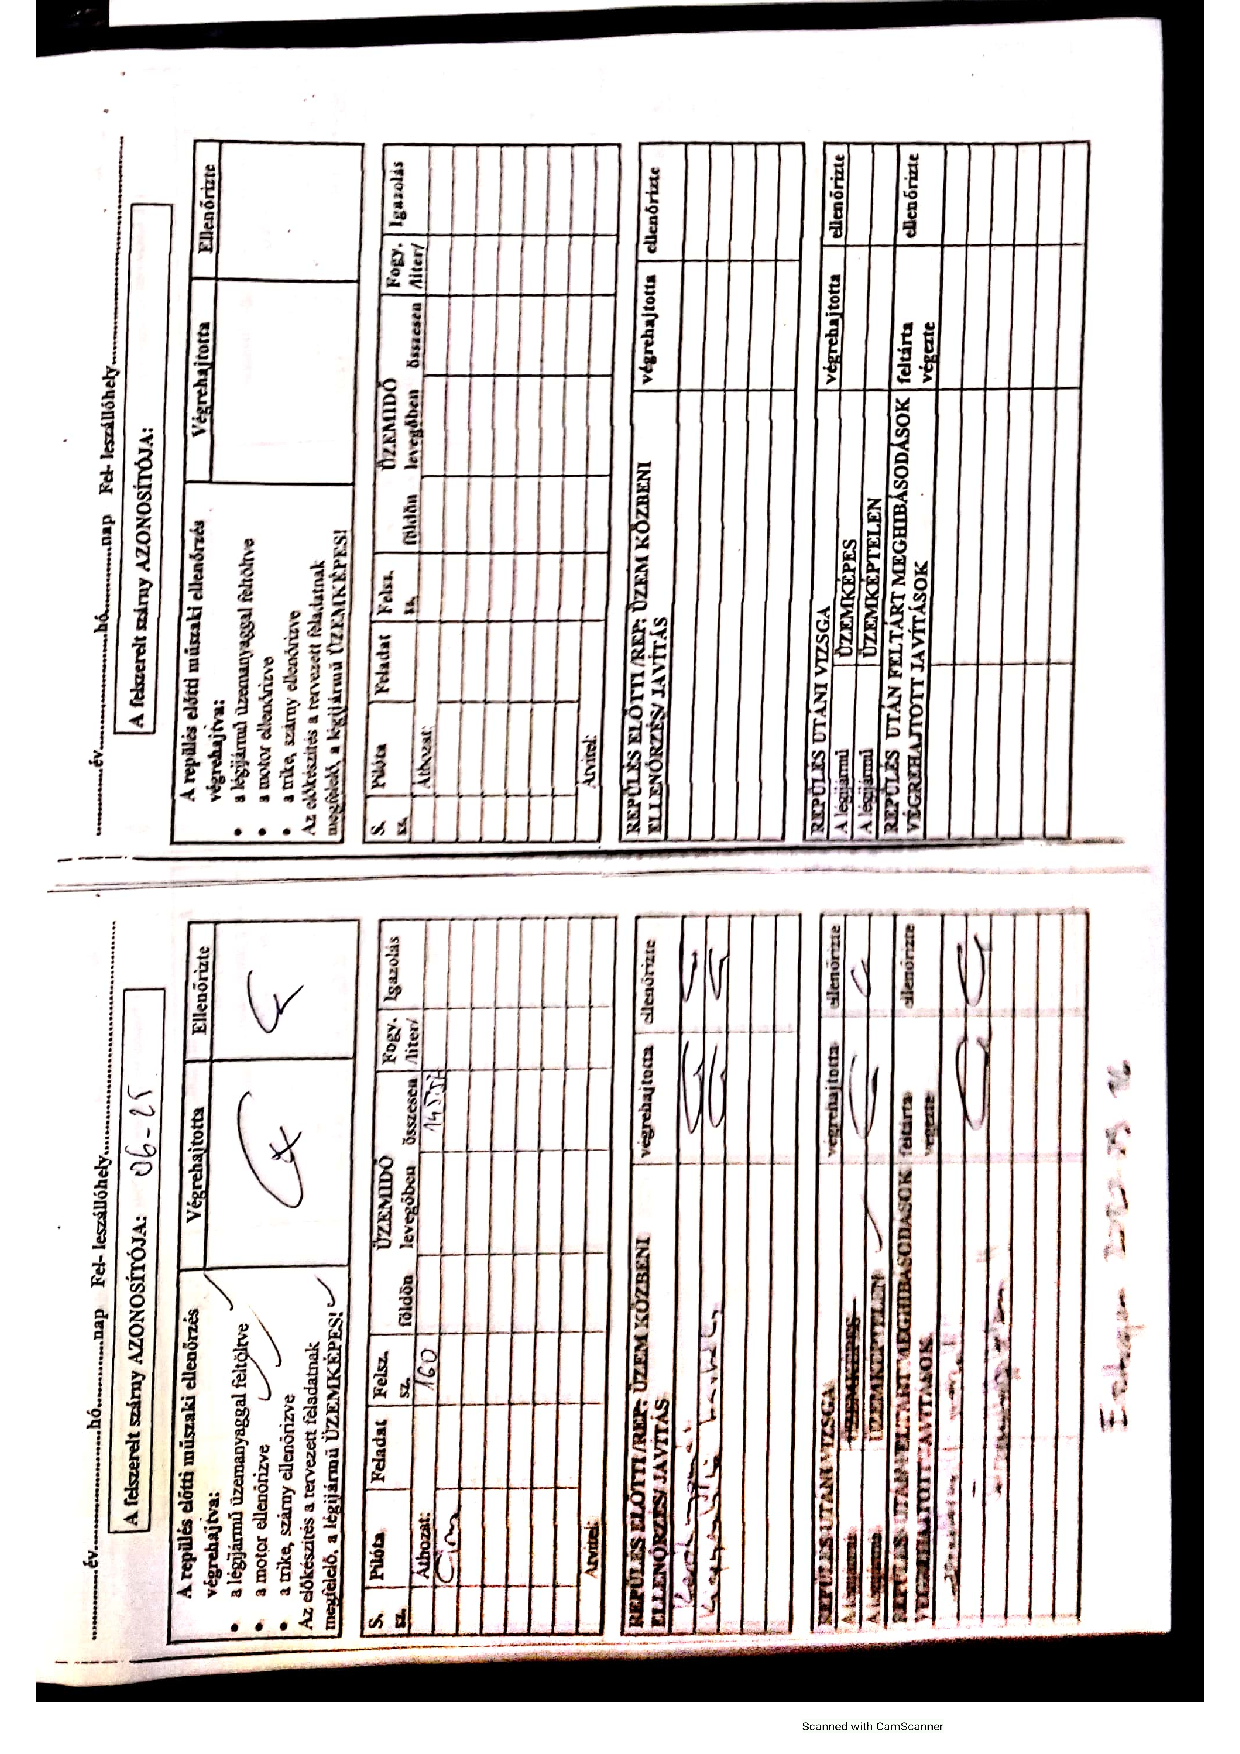
\includepdf[scale=0.70, page={1,3,4}, pagecommand=\section*{1. számú 
melléklet}]{pdf/1-okmanyok}

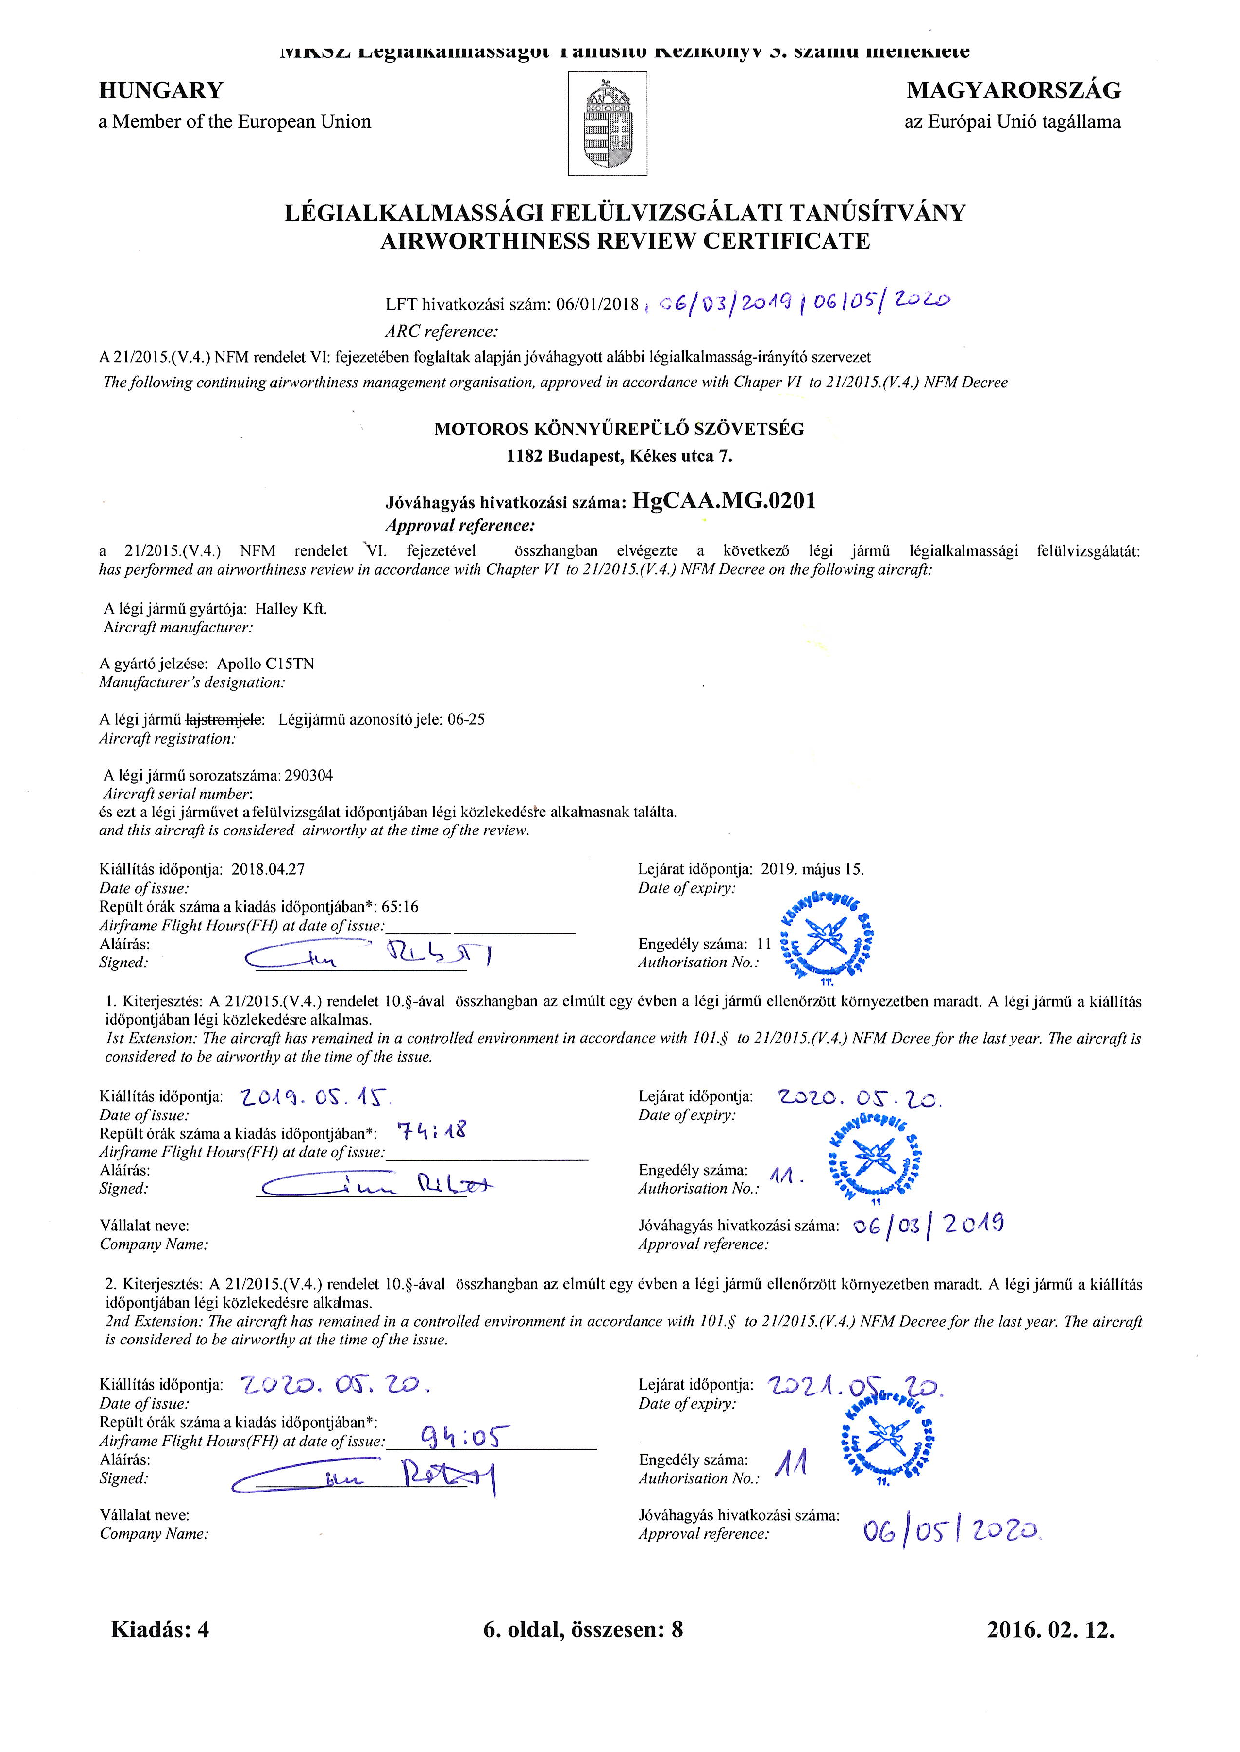
\includepdf[scale=0.75, pagecommand=\section*{2. számú melléklet}]{pdf/2-alktan}

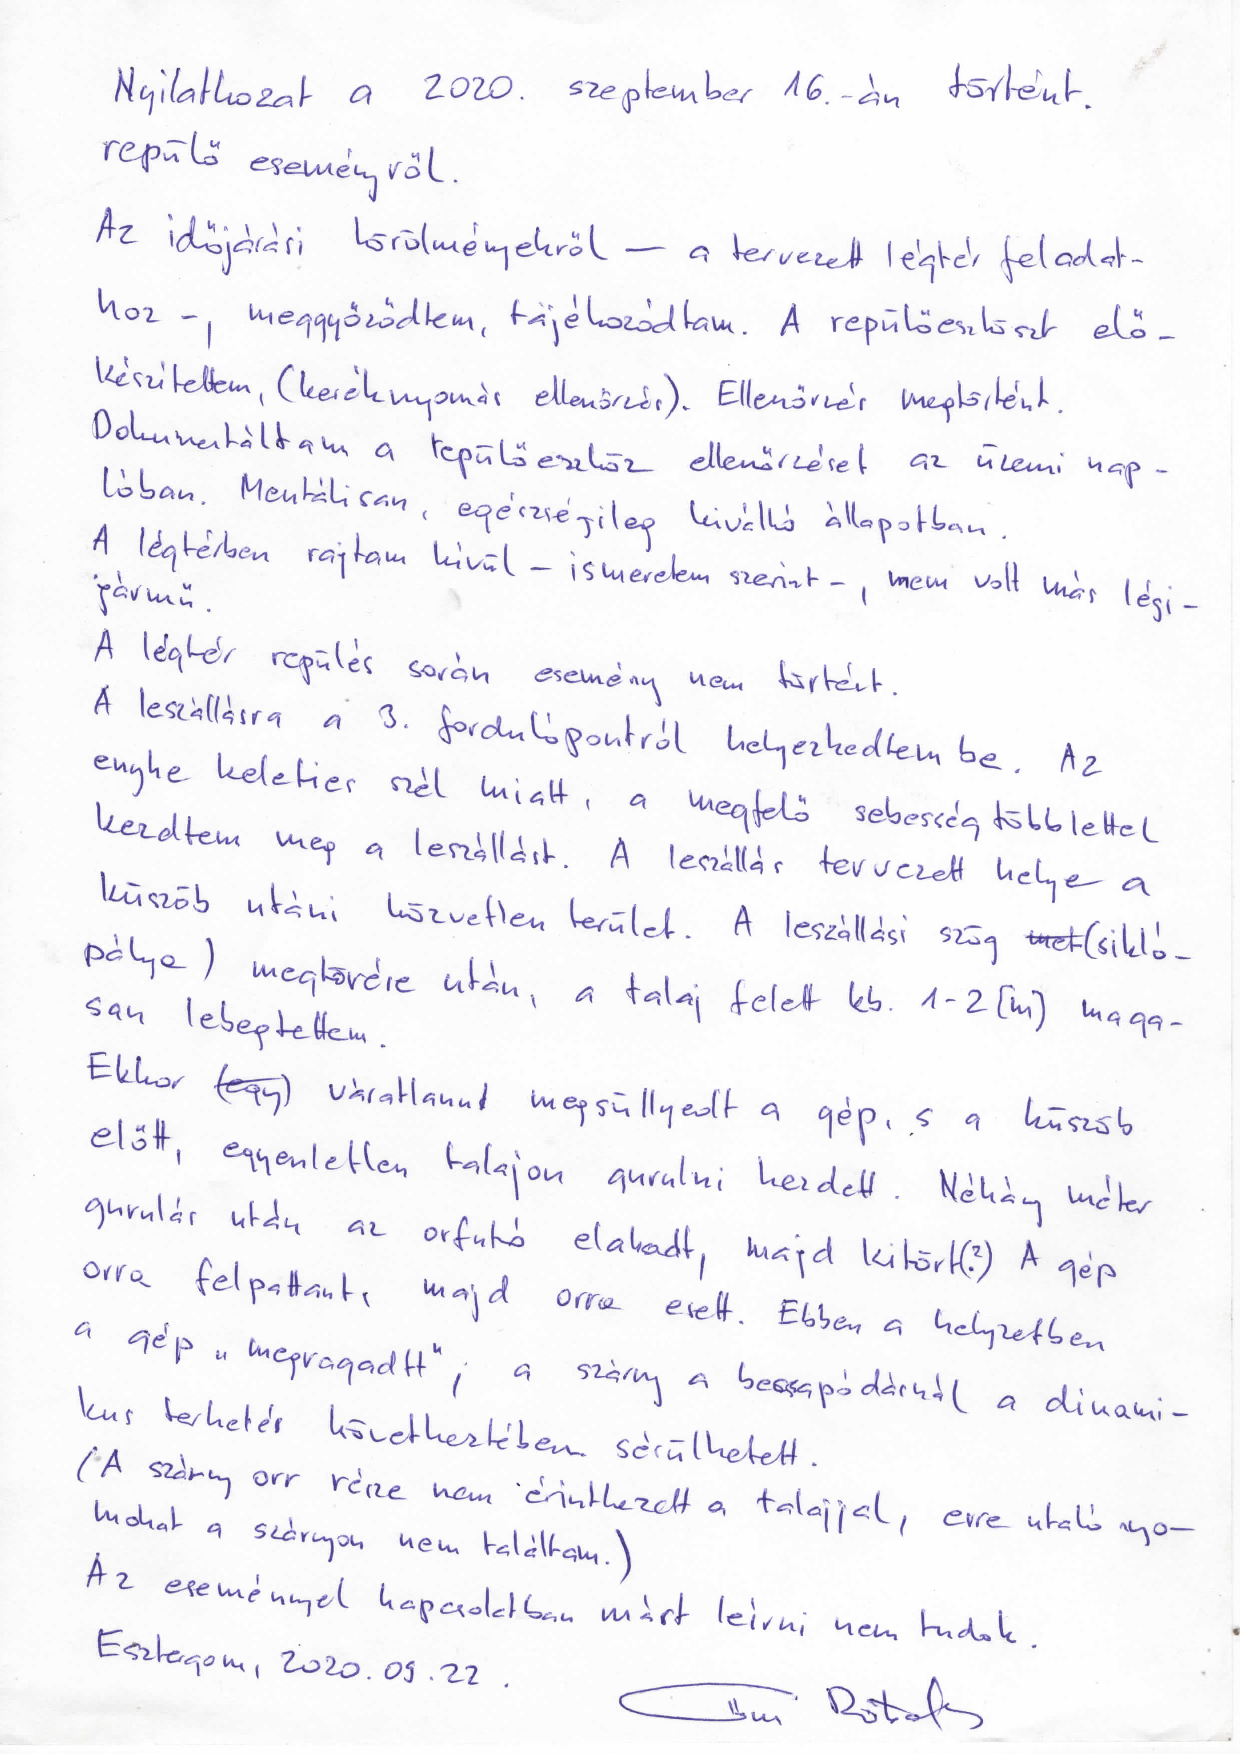
\includepdf[scale=0.75, pagecommand=\section*{3. 
számú melléklet}]{pdf/3-pilotanyilatkozat}

\pagebreak
\section*{4. számú melléklet}
\begin{figure}[ht!]
\centering
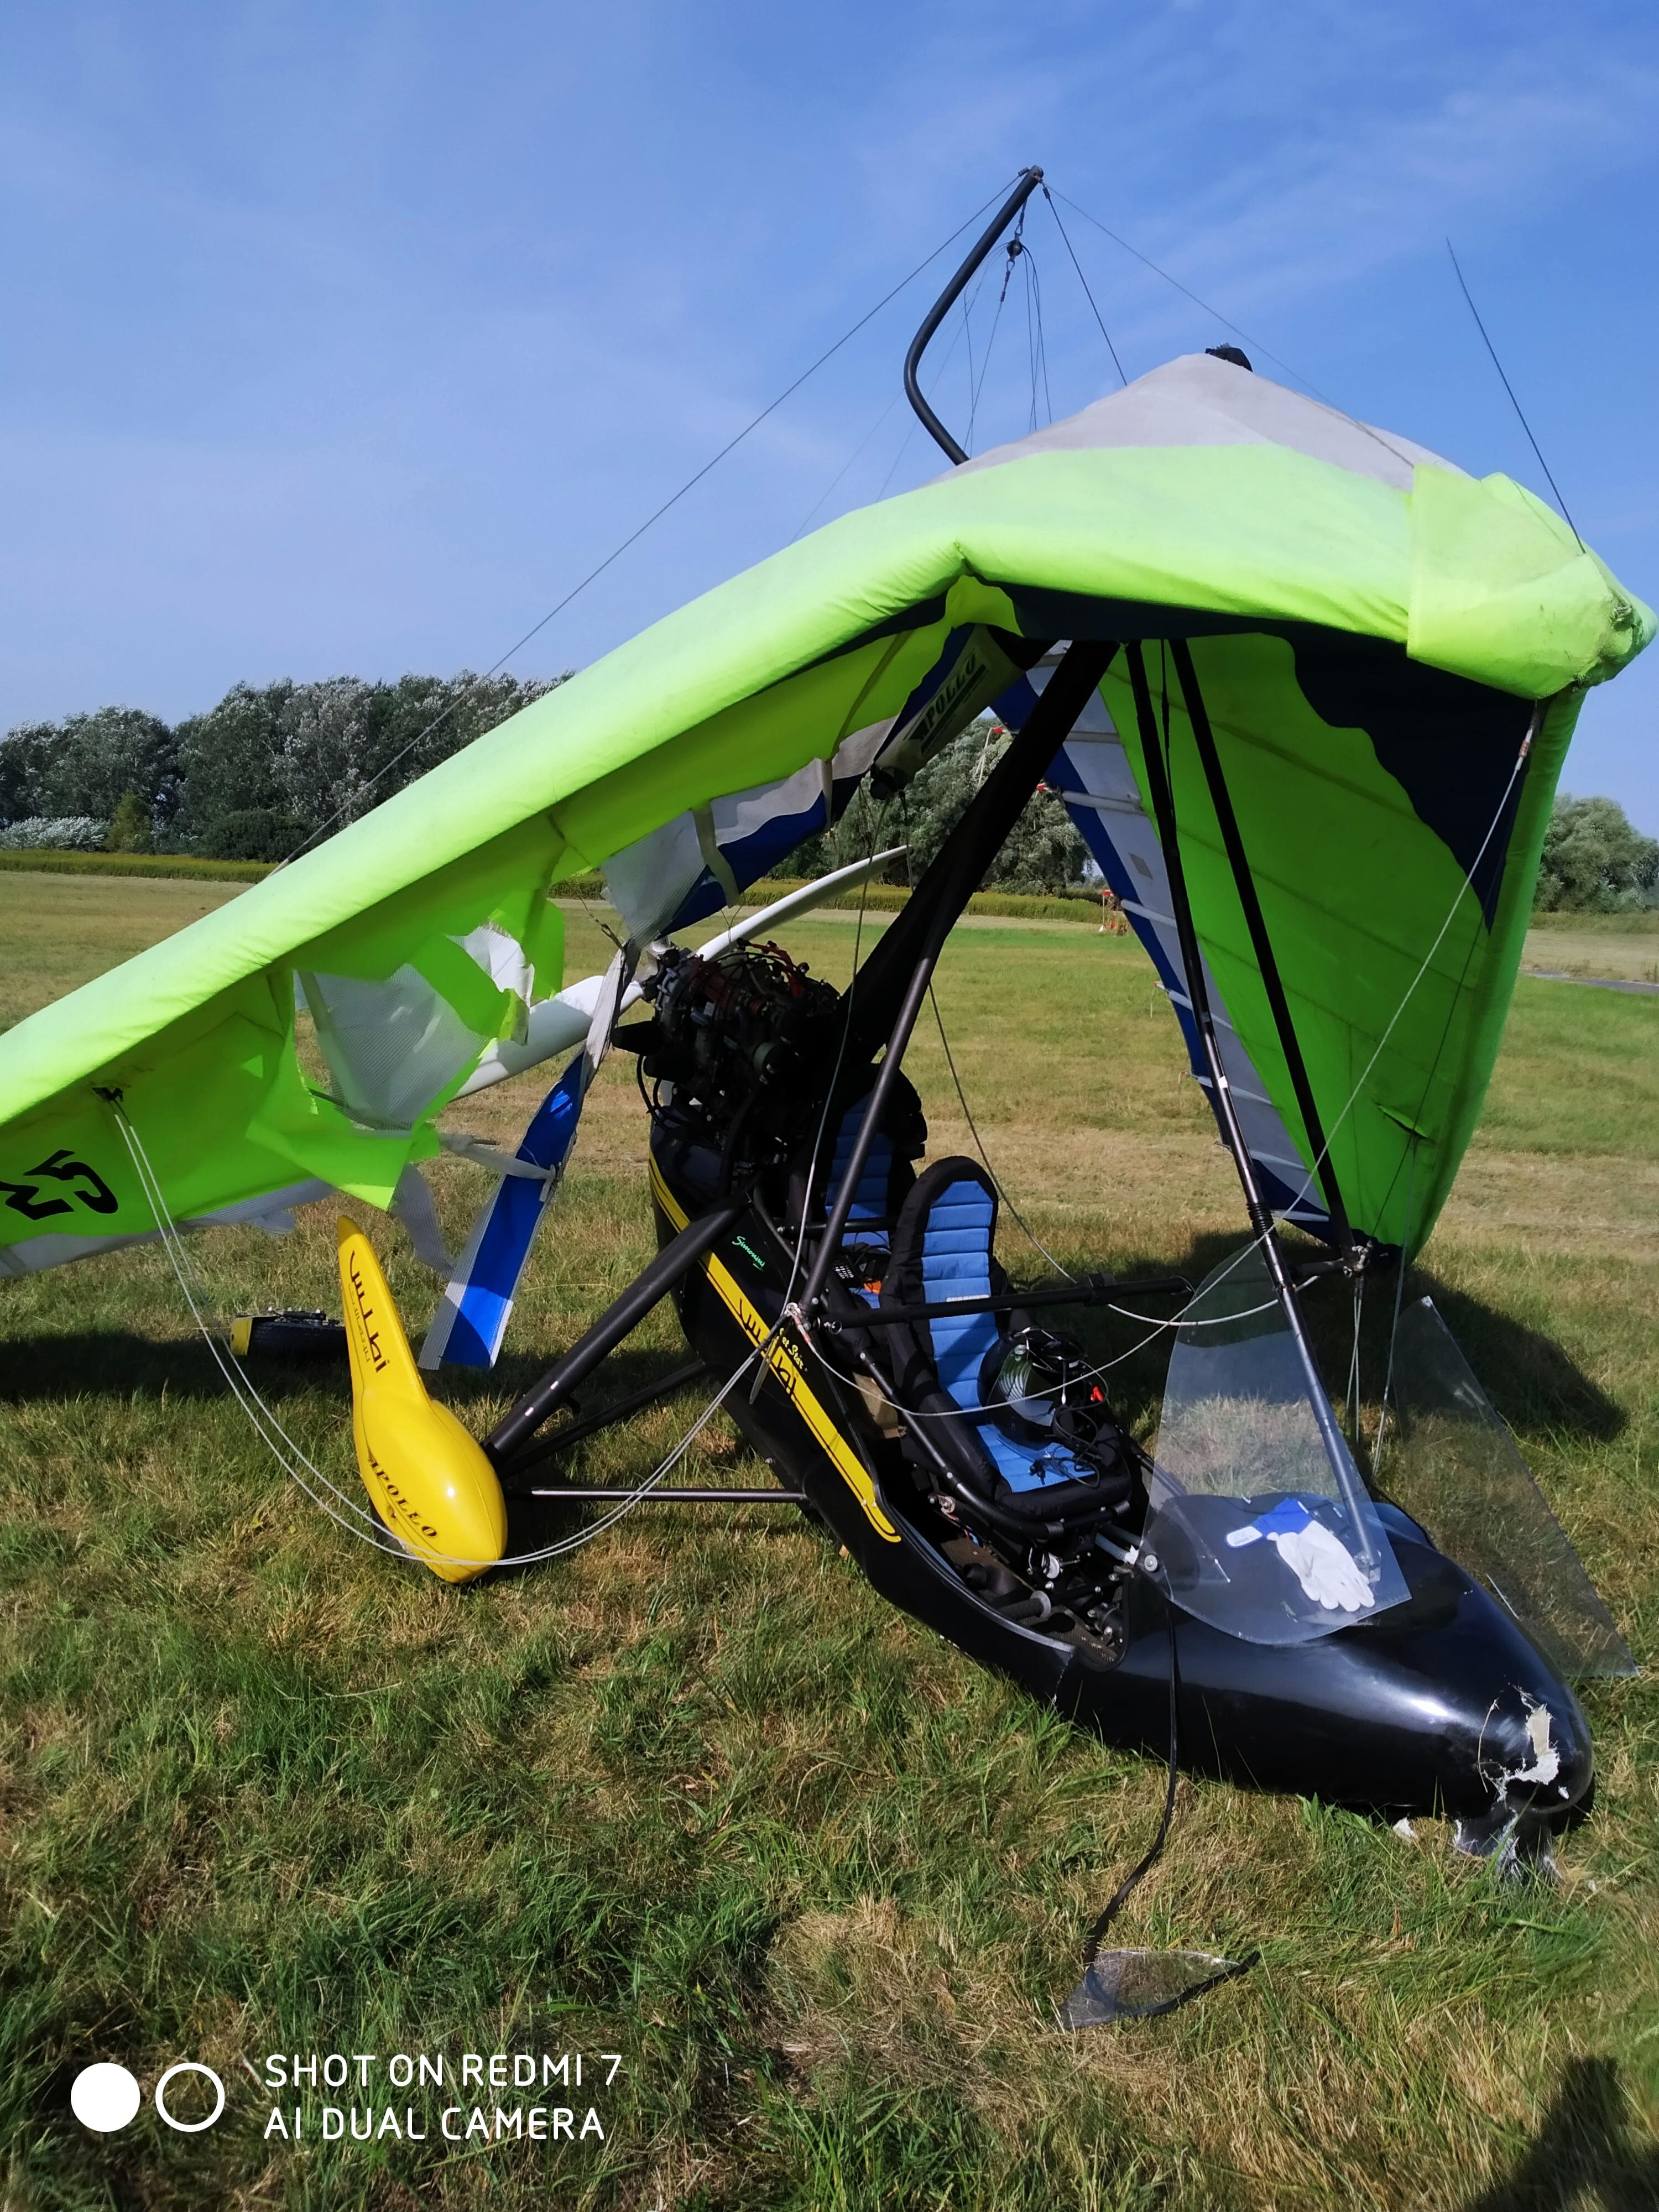
\includegraphics[width=13cm]{kepek/CR1}
\end{figure}
\begin{figure}[ht!]
\centering
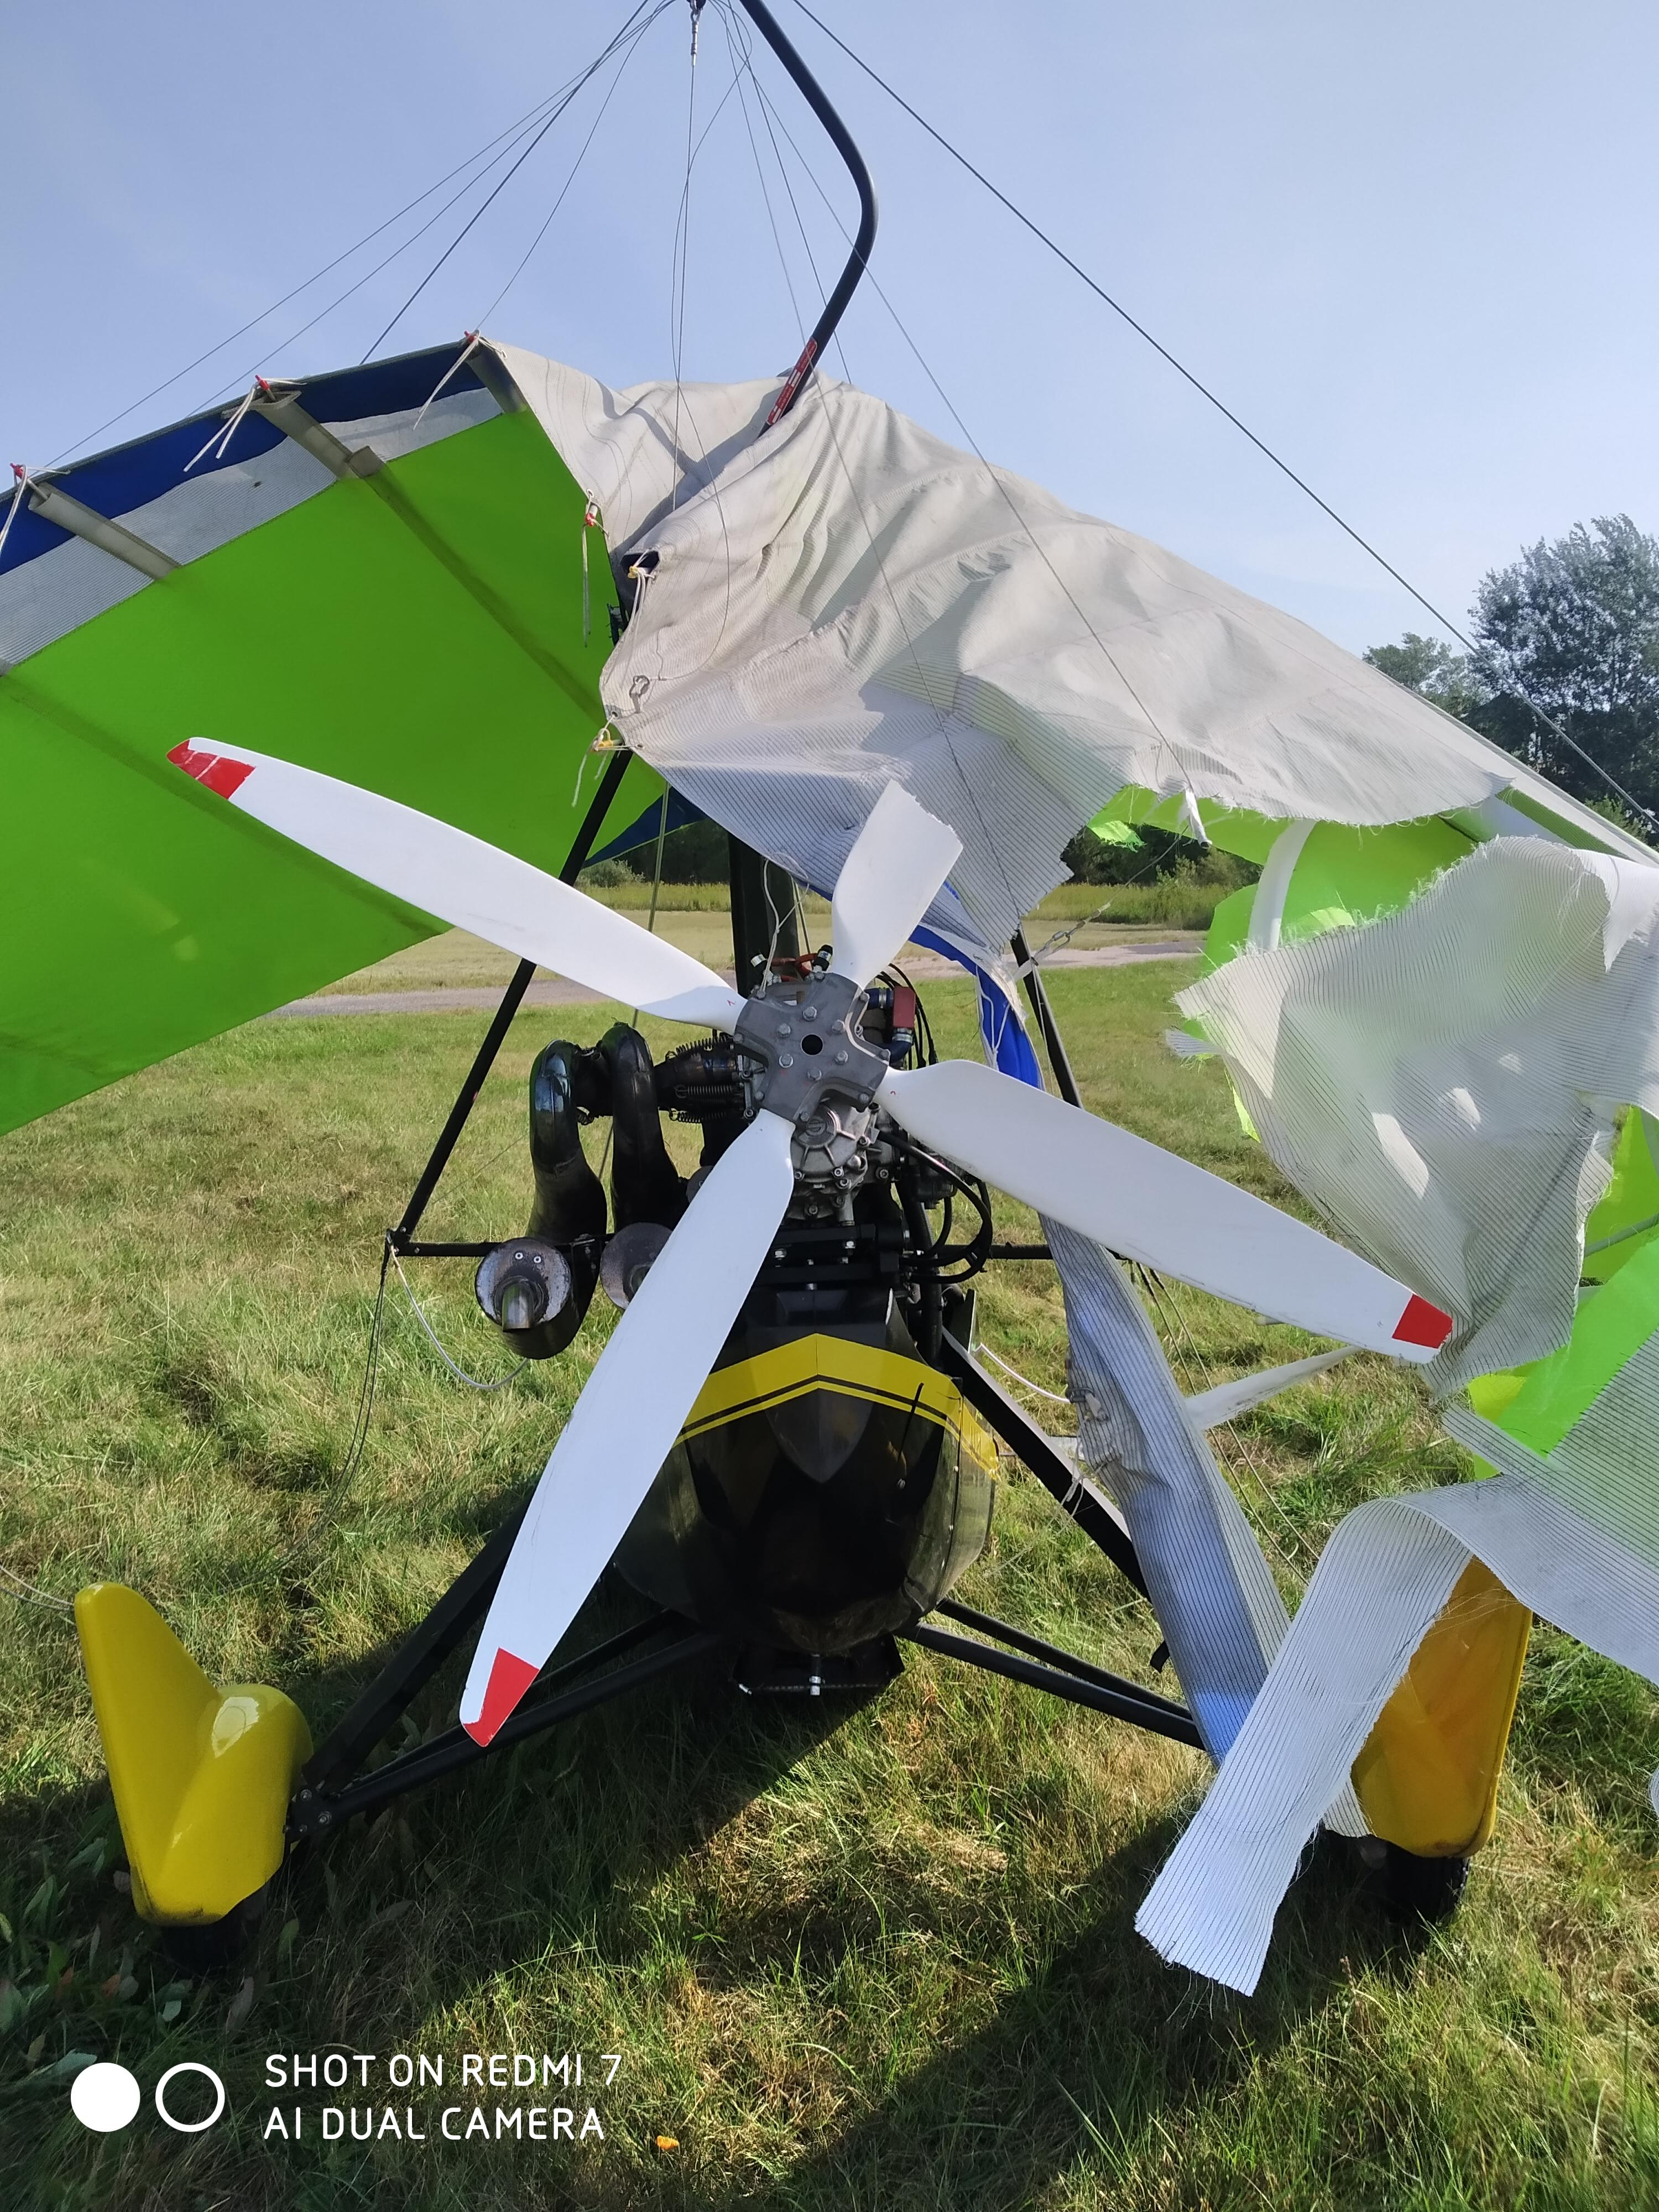
\includegraphics[width=13cm]{kepek/CR2}
\end{figure}
\begin{figure}[ht!]
\centering
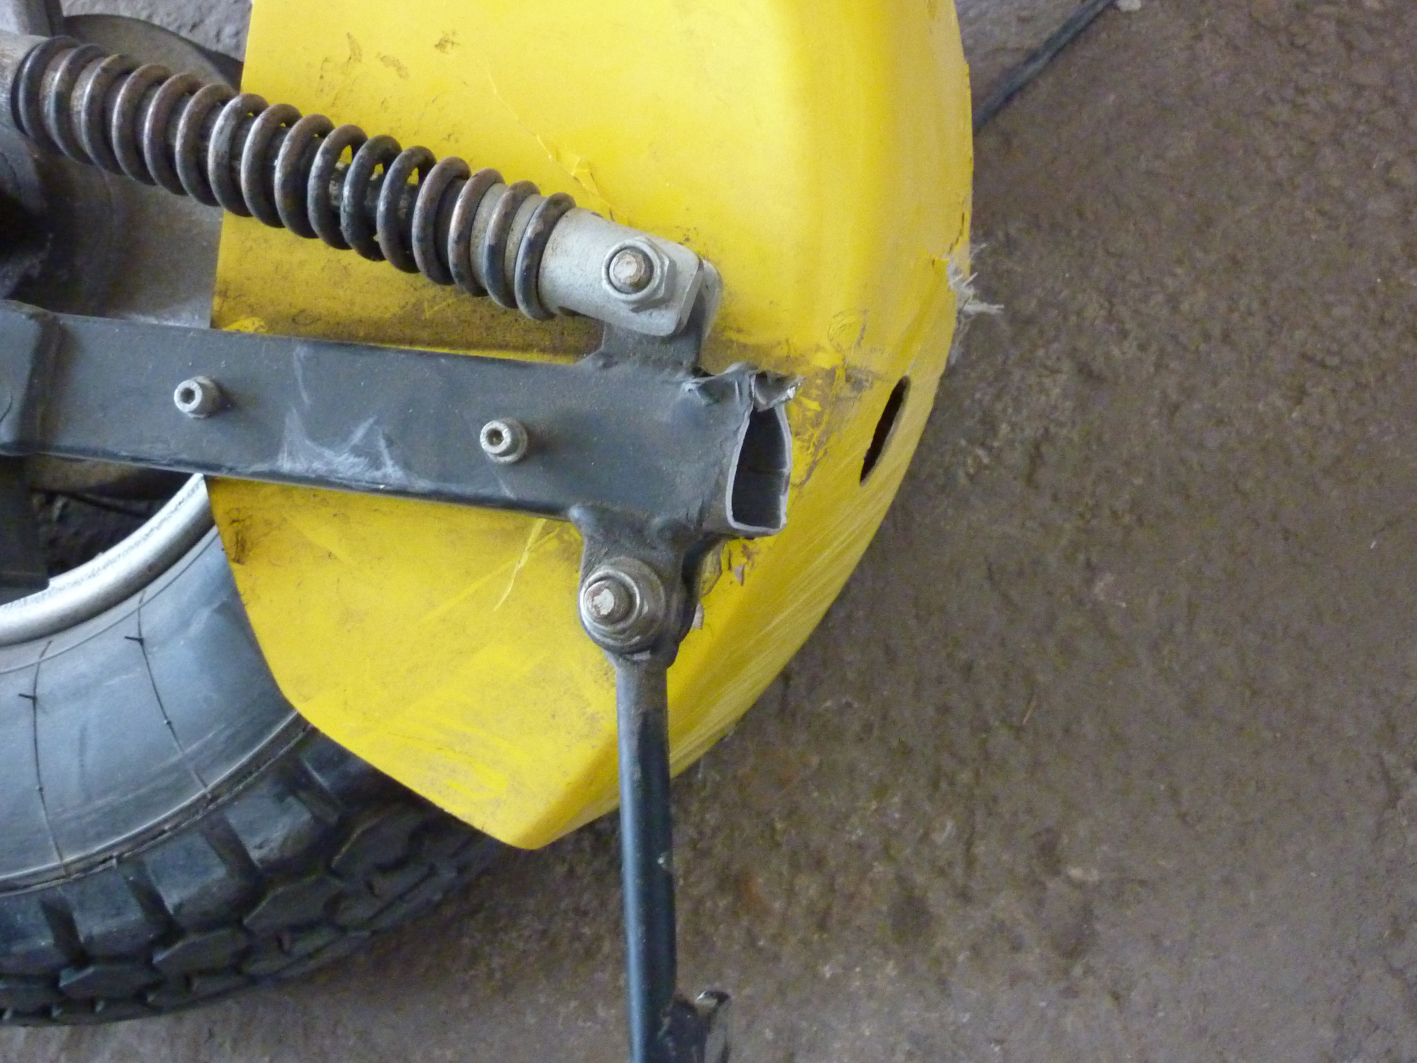
\includegraphics[width=13cm]{kepek/KJ1}
\end{figure}
\begin{figure}[ht!]
\centering
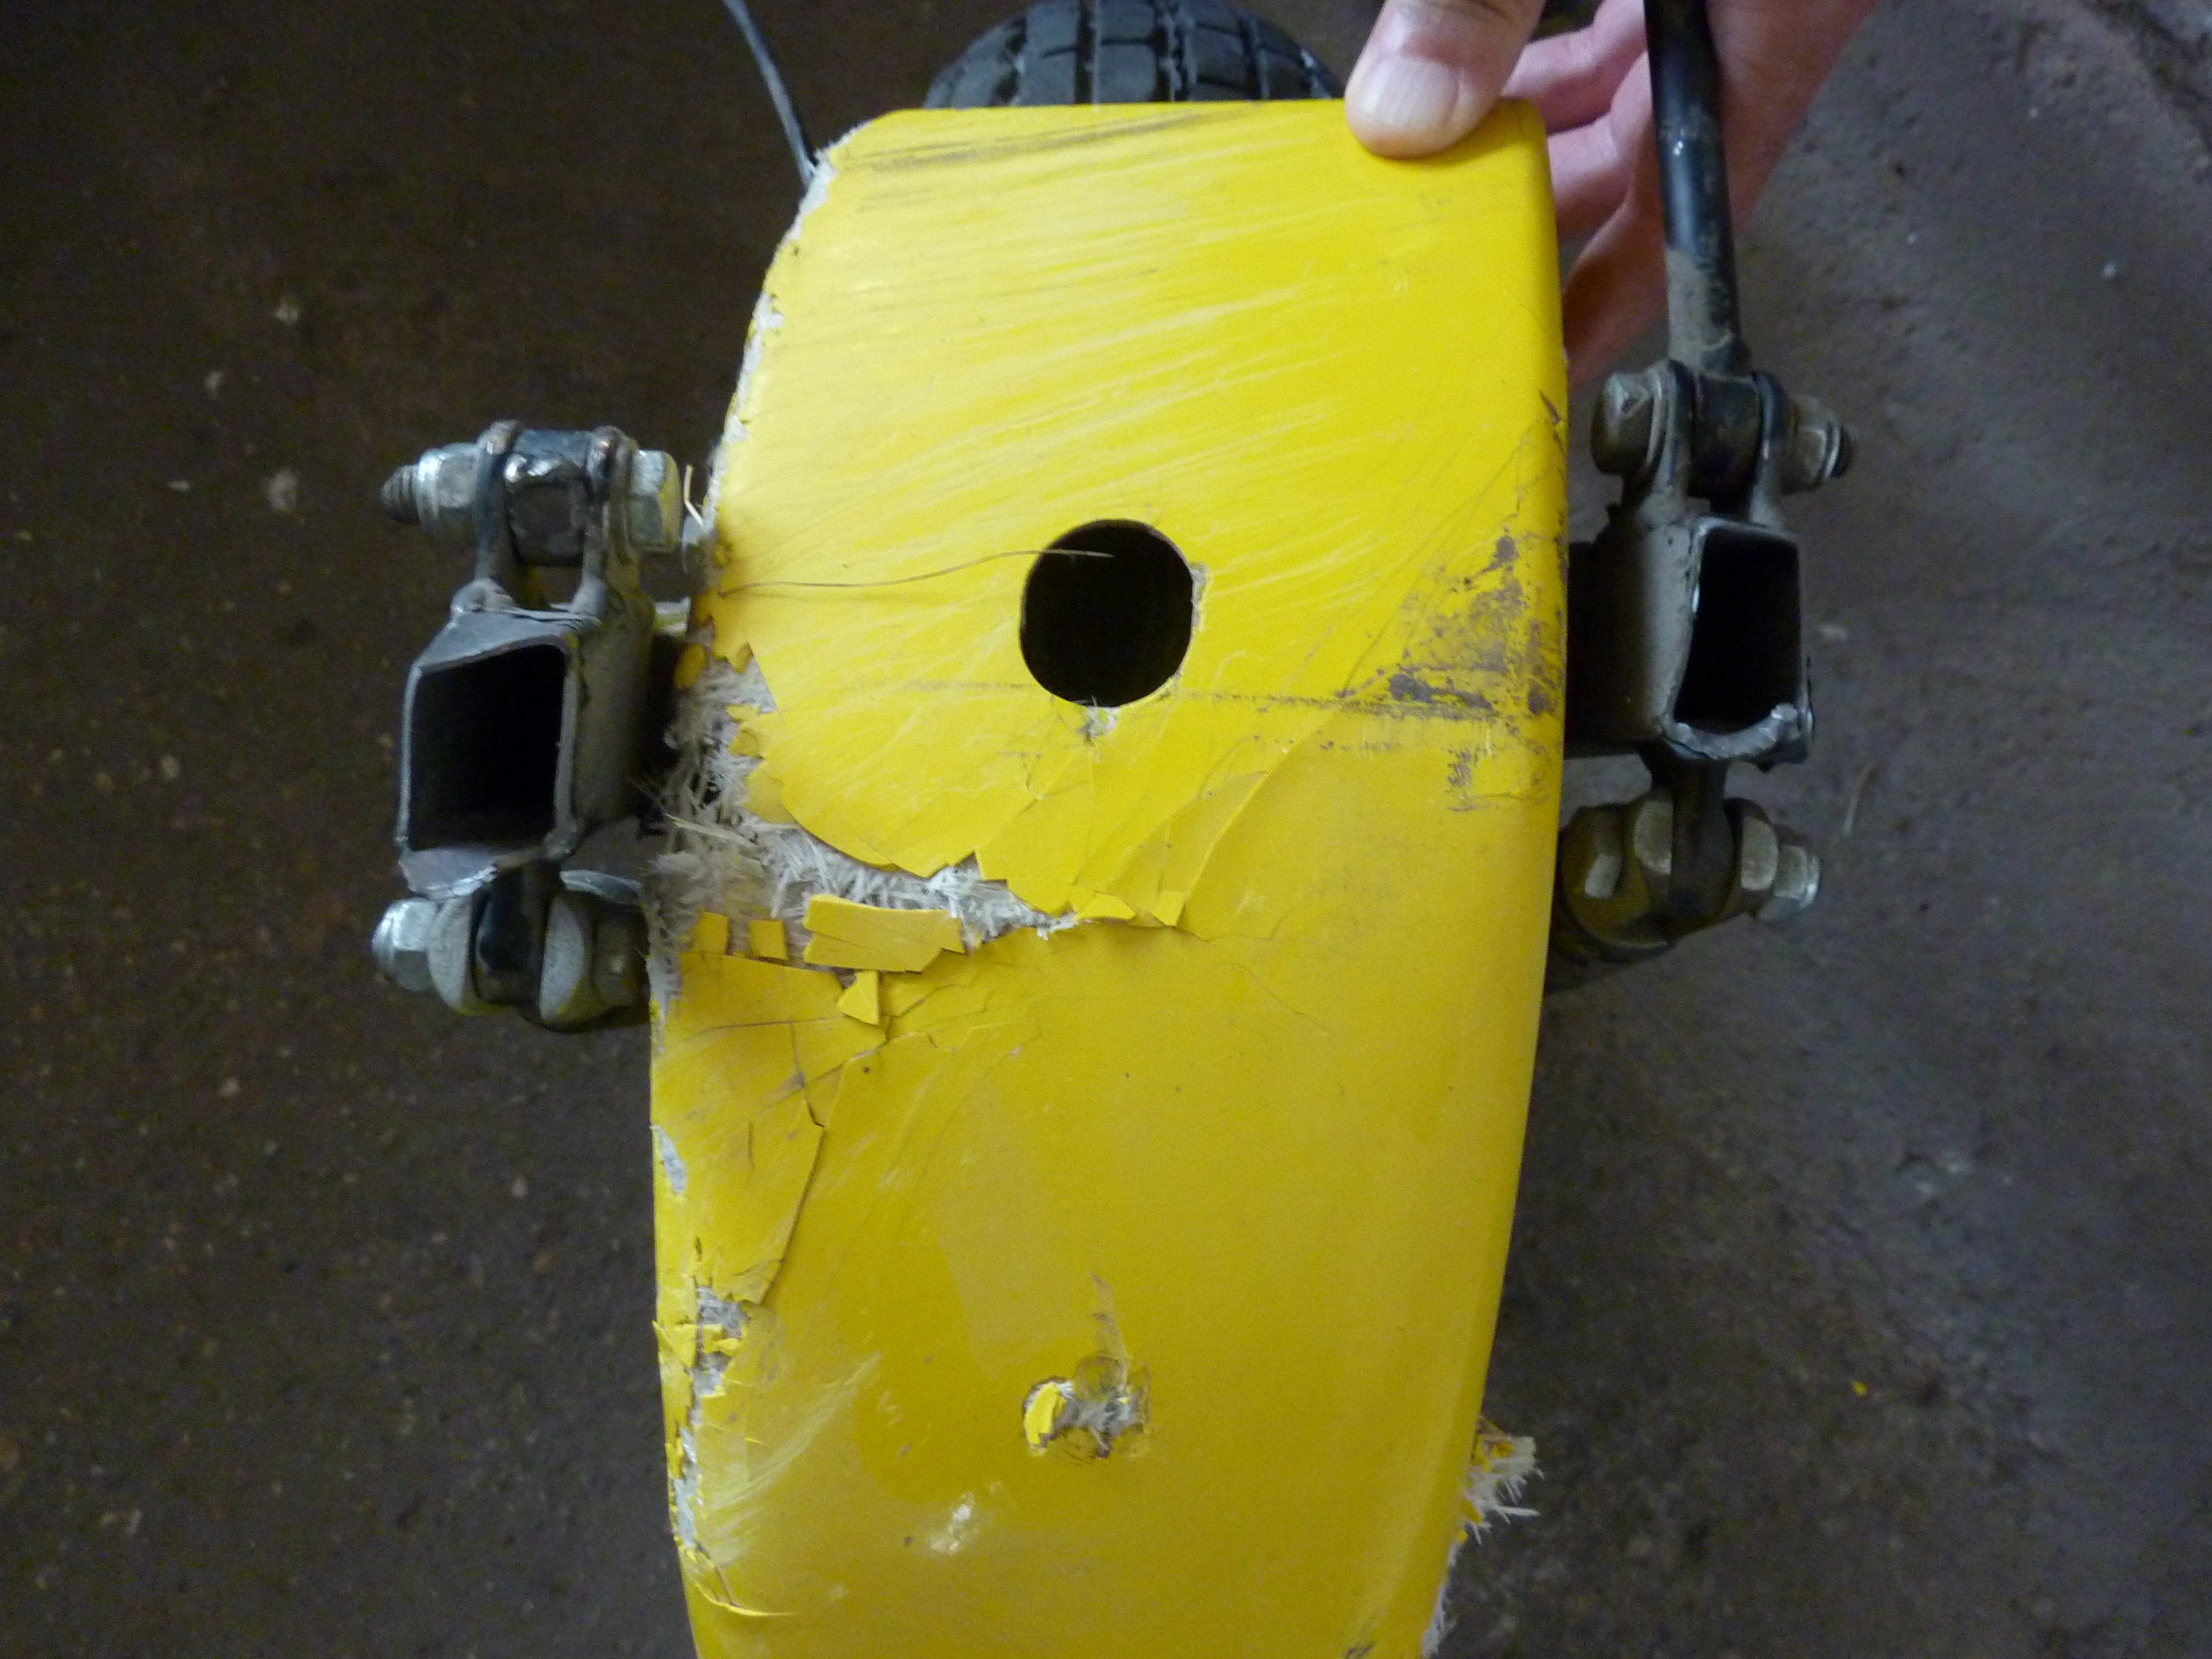
\includegraphics[width=13cm]{kepek/KJ3}
\end{figure}
\begin{figure}[ht!]
\centering
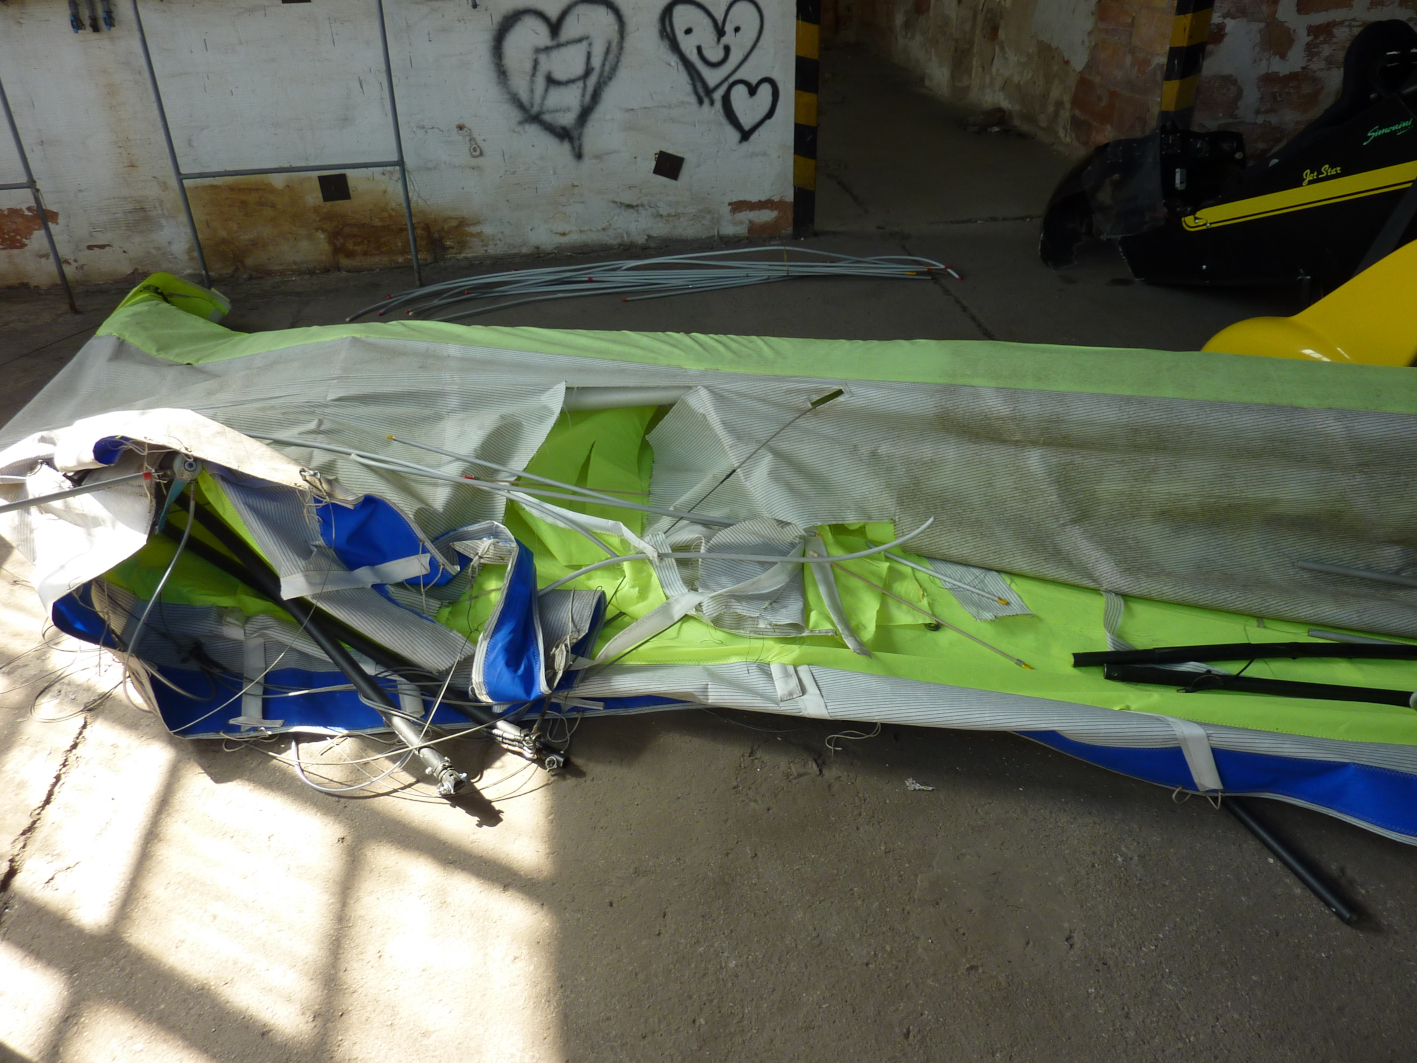
\includegraphics[width=13cm]{kepek/KJ2}
\end{figure}
\begin{figure}[ht!]
\centering
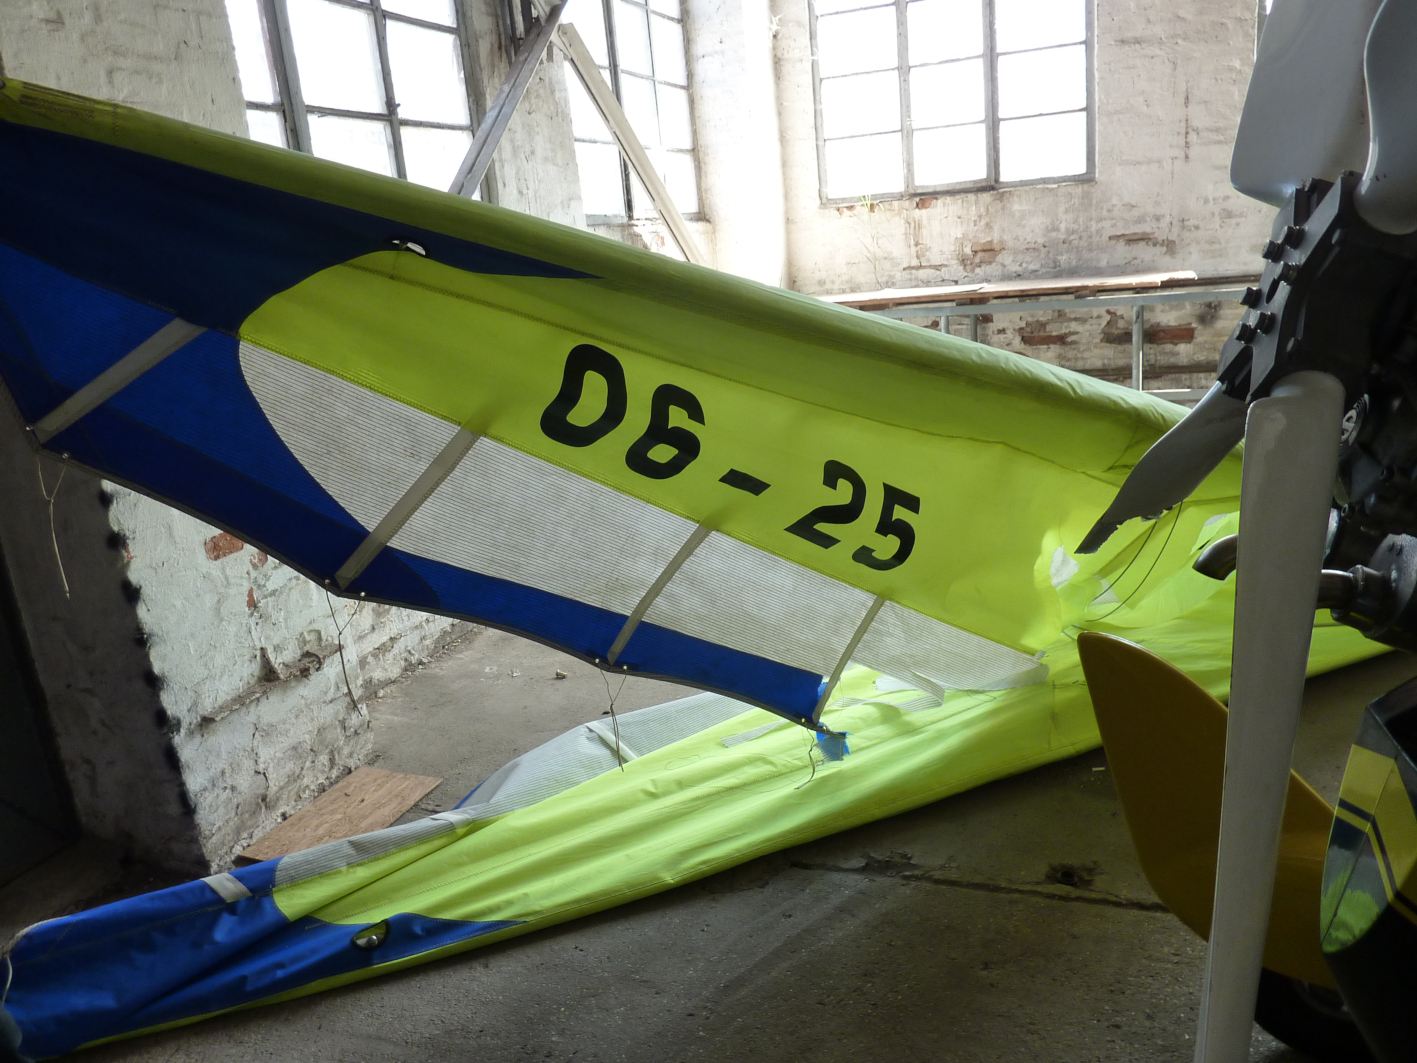
\includegraphics[width=13cm]{kepek/KJ4}
\end{figure}
\begin{figure}[ht!]
\centering
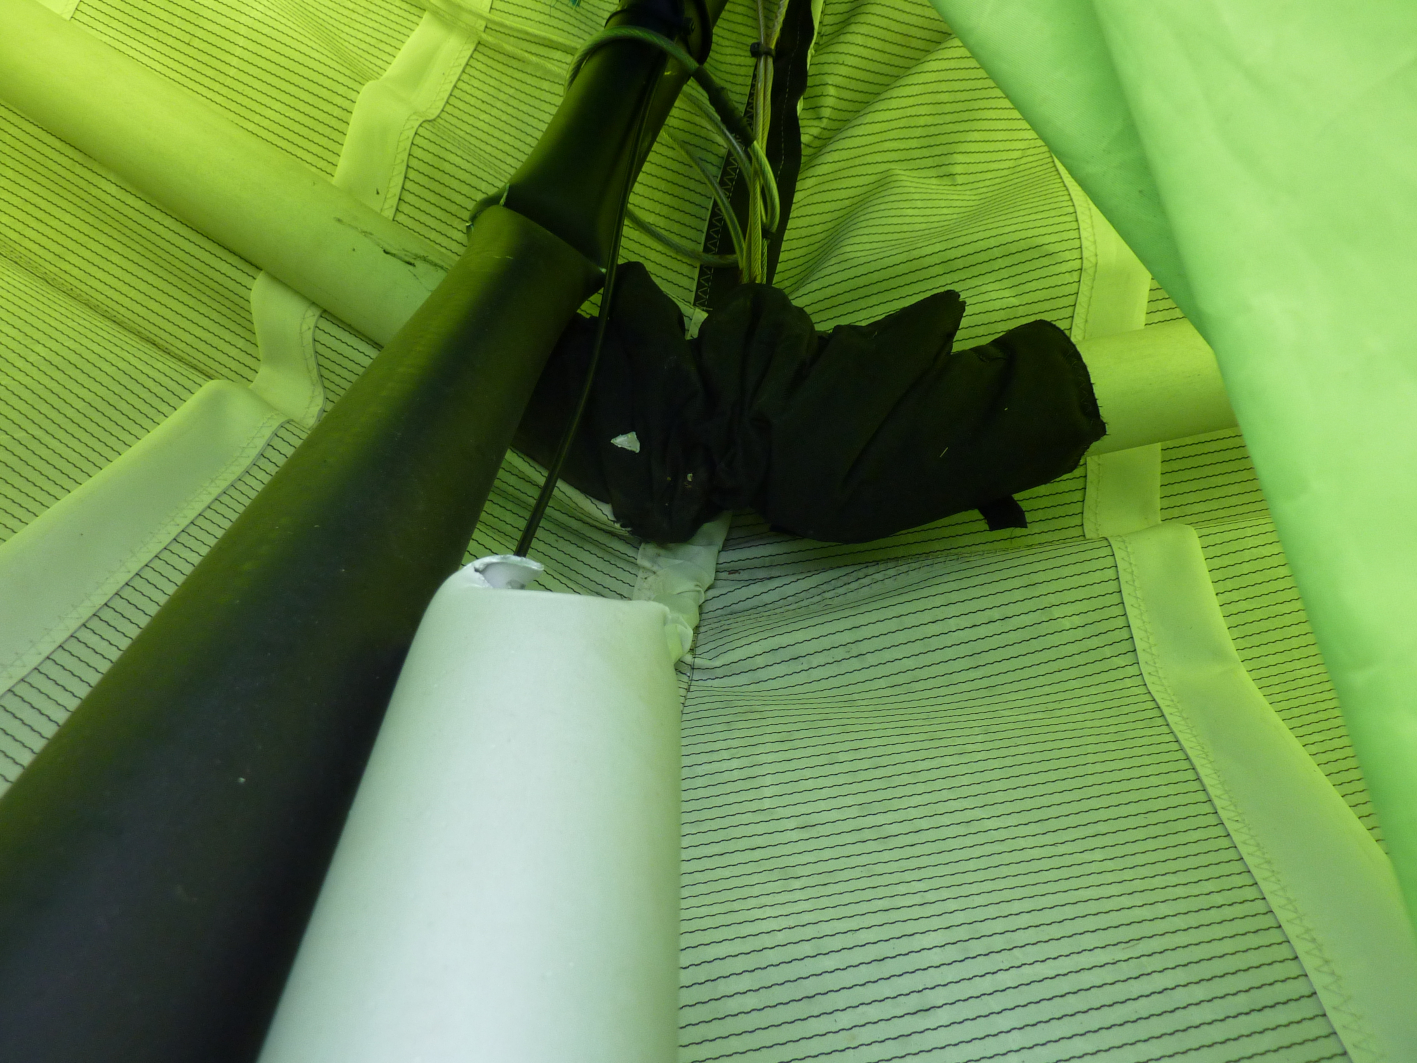
\includegraphics[width=13cm]{kepek/KJ5}
\end{figure}
\begin{figure}[ht!]
\centering
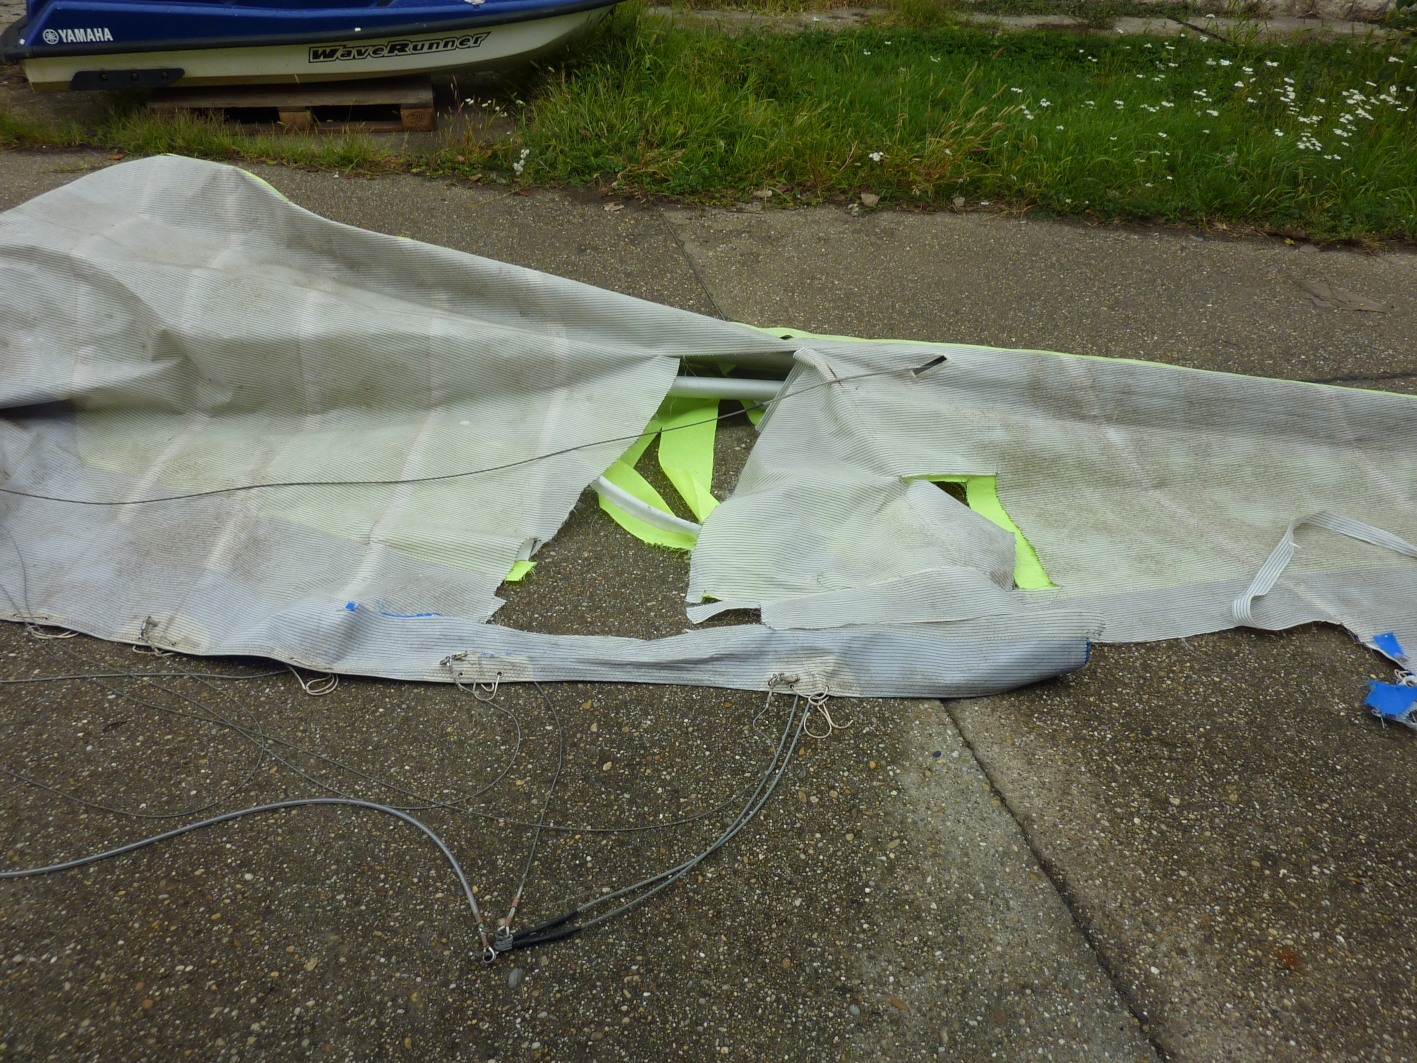
\includegraphics[width=13cm]{kepek/KJ6}
\end{figure}


%
%%
%%%
%%
% 
\end{document}
